\chapter{Project Design}

\section{Proposed System}
In this project we will be using abstractive approach to summarize the text. We would create our own model and integrate it with the website to provide user-friendly interface. 
Users can generate the summary by adding text or by uploading files.  
Non-registered users can summarize the text with specific word and usage limit.
Whereas, registered users would have the benefit of summarizing the text without any usage limit and their summary would be saved in the database for a week so that they can revisit and access their summarized text.

\section{Design (Flow of Modules) \& Class Diagram}
\begin{figure}[h]
\centering
\scalebox{0.7}{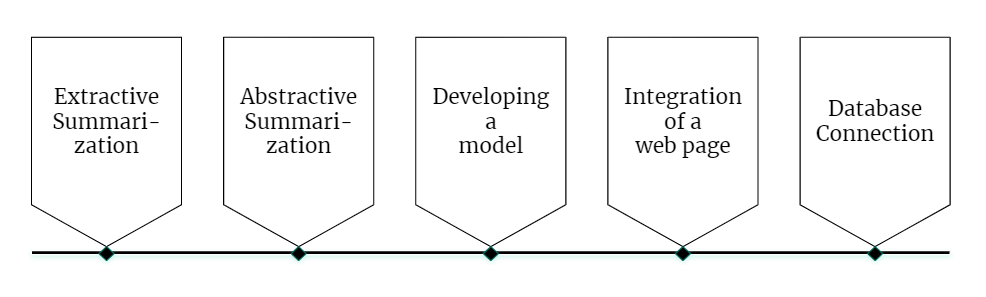
\includegraphics{design_flow.png}}
\caption{Flow of Modules}
\label{Flow of Modules}
\end{figure}
As shown in the Fig. 3.1, both extractive and abstractive summarization approaches will be implemented in this project, and in the order represented in the figure. AAbstractive summarization will be used for actual text summarization whereas extractive text summarization will be used for generation of notes. A ML model will be designed on successful completion of abstractive summarization. To provide User Interface (UI) we will integrate a web page with the ML model and add database connectivity to store the user credentials and their activity on the website.
\begin{figure}[h]
\centering
\scalebox{0.7}{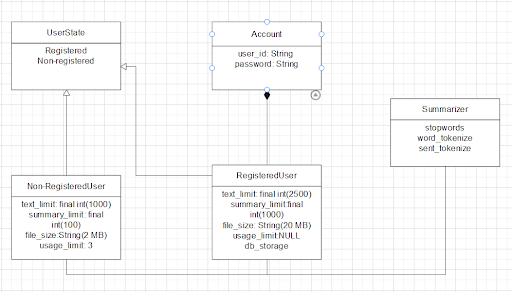
\includegraphics{class_diag.png}}
\caption{Class Diagram Model}
\label{Class Diagram Model}
\end{figure}

\section{Modules}
\subsection{Module 1: User State (Web Page)}
Whenever the application will be accessed, login status will be checked.
If login hasn’t been done then the user will be able to access only few of the features of the application.
Upon logging in, the registered user can access additional features, helpful for summarization of text.

\subsection{Module 2: Non-Registered User}
If any user hasn’t logged in or hasn’t registered, they will be able to use the application but with few restrictions.
A limit will be set in terms of number of words for adding text for which summarization is required. (word limit: 1000)
Similarly a limit for summarized text will also be applied. (word limit: 100)
For non-registered users, there will also be a usage limit i.e. they can use the tool only thrice after which they will have to register if the wish to continue using the application.

\subsection{Module 3: Account}
If users decides upon creating an account they have to go through registering activity.
A SQL database will be connected to the web page which will store the user’s credentials upon generation of an account.
Then the user can login through their credentials and access the account.
With the help of an account, the user can track their previous work easily.

\subsection{Module 4: Registered User}
Once logging activity is done user can access additional features and summarize more text.
The limit for input text and summarized text will be increased.
There will be no limit to the number of times a user can use the tool for summarizing text passages.
We also wish to add the feature of storing the summarized text for 7 days after which it will be erased from the database. The user can revisit the application and access the summarized text generated within last 7 days.


\section{References}
\begin{itemize}
    \item Title of the paper : Text summarization using neural networks
Authors : Mr Anish Jadhav, Mr Rajat Jain, Mr Steve Fernandes, Mrs Sana Shaikh 
Year of publication : 2018
\item Title : Extractive text summarization using sentence ranking
Authors : Mrs J.N.Madhuri, Mr Ganesh Kumar
Year of publication : 2019
\item Title : An overview on extractive text summarization
Authors : Mr Shohreh Rad Ramini, Mr Ali Toofanzahdeh Mozhdehi
Year of publications : 2017
\item https://medium.com/analytics-vidhya/simple-text-summarization-using-nltk-eedc36ebaaf8
\item https://stackabuse.com/text-summarization-with-nltk-in-python/
\item https://towardsdatascience.com/a-quick-introduction-to-text-summarization-in-machine-learning-3d27ccf18a9f
\item https://www.analyticsvidhya.com/blog/2018/11/introduction-text-summarization-textrank-python/

\end{itemize}



